\documentclass[12pt]{article}
\usepackage[left=0.25cm,top=1cm,right=0.25cm,bottom=1cm]{geometry}
\textwidth = 20cm
\hoffset = -1cm
\usepackage[utf8]{inputenc}
\usepackage[spanish,es-tabla]{babel}
\usepackage[autostyle,spanish=mexican]{csquotes}
\usepackage[tbtags]{amsmath}
\usepackage{nccmath}
\usepackage{amsthm}
\usepackage{amssymb}
\usepackage{graphicx}
\usepackage{standalone}
\usepackage[outdir=./]{epstopdf}
\usepackage{siunitx}
\usepackage{physics}
\usepackage{color}
\usepackage{float}
\usepackage{multicol}
%\usepackage{milista}
\usepackage{enumitem}
\usepackage{anyfontsize}
\usepackage{anysize}
\usepackage{enumitem}
\usepackage{capt-of}
\usepackage{bm}
\usepackage{relsize}
\usepackage{placeins}
\usepackage{empheq}
\usepackage{cancel}
\usepackage{wrapfig}
\spanishdecimal{.}
\renewcommand{\baselinestretch}{1.5} 
\renewcommand\labelenumii{\theenumi.{\arabic{enumii}}}
\newcommand{\ptilde}[1]{\ensuremath{{#1}^{\prime}}}
\newcommand{\stilde}[1]{\ensuremath{{#1}^{\prime \prime}}}
\newcommand{\ttilde}[1]{\ensuremath{{#1}^{\prime \prime \prime}}}
\newcommand{\ntilde}[2]{\ensuremath{{#1}^{(#2)}}}


\title{Ejercicios para el Tema 4 \\[0.3em]  \large{Matemáticas Avanzadas de la Física}\vspace{-3ex}}
\author{M. en C. Gustavo Contreras Mayén}
\date{ }
\begin{document}
\vspace{-4cm}
\maketitle
\fontsize{14}{14}\selectfont

\textbf{Indicaciones: } Deberás de resolver cada ejercicio de la manera más completa, ordenada y clara posible, anotando cada paso así como las operaciones involucradas.

\begin{enumerate}
%Ref. Arfken (2006) 12.1.3
\item Demuestra que el potencial electrostático producido por una carga $q$ en $z = a$ para $r < a$ es:
\begin{align*}
\varphi(\vb{r}) = \dfrac{q}{4 \pi \epsilon_{0} a} \, \nsum_{n=0}^{\infty} \left( \dfrac{r}{a} \right)^{n} \, P_{n}(\cos \theta)
\end{align*}
\item Una esfera conductora de calor de radio $a$ está compuesta por dos hemisferios con un espacio infinitesimal aislante entre ellos, como se muestra en la figura (\ref{fig:figura2}).
\begin{figure}[H]
    \centering
   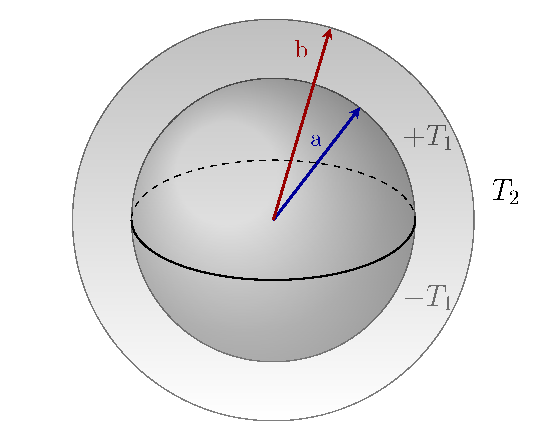
\includegraphics[scale=0.9]{Imagenes/esfera1.eps}
    \caption{Los hemisferios de la esfera interior se encuentran a diferentes temperatura.}
    \label{fig:figura2}
\end{figure}
Las mitades superior e inferior de la esfera están en contacto con baños térmicos de temperaturas $+ T_{1}$ y $-T_{1}$, respectivamente. La esfera de radio $a$ está dentro de otra esfera conductora de calor de radio $b$ con una temperatura $T_{2}$.
Calcula la temperatura:
\begin{enumerate}[label=\roman*)]
\item Dentro de la esfera interior,
\item En la región entre las dos esferas, y
\item Por fuera de la esfera exterior.
\end{enumerate}
%Ref. Boas (20059 Chapter 12. Problems 10, 12)
\item Expande en términos de una serie con Polinomios de Legendre los siguientes polinomios:
\begin{enumerate}[label=\alph*)]
\item $3 \, x^{2} + x - 1$
\item $x - x^{3}$
\end{enumerate}
\end{enumerate}
\end{document}